\chapter{Signal extraction}
In this chapter the procedure for signal yield extraction is presented. We use the framework of \texttt{RooFit} \cite{verkerke2006roofit} where we define 2D histogram templates in \vars, based on MC, for signal and several types of background. Using these templates, the independent full sample is fitted with binned extended maximum likelihood (ML) fit, so that the individual template ratios and their sum describe the fitted sample as best as possible. In particle physics we are often dealing with low numbers of events and need to account for the Poisson nature of the data, therefore we use the likelihood fit, since it takes the Poisson errors into account, unlike the $\chi^2$ fit, where the errors are assumed to be Gaussian. In this procedure we attempt to find the parameter values that maximize the likelihood function, given the observations.

If $P(n\vert\vec \alpha)$ is the probability of measuring $n$ candidates, where $\vec \alpha$ is a set of parameters on which $P$ depends, we can define the likelihood function $L$ for a series of such measurements (i.e., bins in histogram) $n_i$ based on Poisson statistics as
\begin{equation}
\label{eq:ML}
L(\vec \alpha) = \prod_{i=1} P(n_i|\vec \alpha) = \prod_{i=1} \frac{\mu_i^{n_i}\mathrm{e}^{-\mu_i}}{n_i!},
\end{equation}
where $\mu_i$ is the expected value for each measurement. It is also common to search for the minimum of the negative value of $\ln L$, or negative log-likelihood (NLL), as
\begin{equation}
\label{eq:NLL}
\mathcal{L}(\vec \alpha) = -\ln L(\vec \alpha) = -\sum_{i}\ln \left(\frac{\mu_i^{n_i}\mathrm{e}^{-\mu_i}}{n_i!}\right) = \sum_{i}\ln(n_i!) + \mu_i - n_i\ln(\mu_i).
\end{equation}
Maximizing $L$ or minimizing $\mathcal{L}$ gives us a maximum likelihood estimate of the set of parameters $\vec \alpha_{ML}$ which best describe the observed data. 

The ML method provides a method to estimate the fit uncertainty. This is especially useful if the log-likelihood has a non-parabolic shape, which leads to asymmetric errors. We calculate the errors using the \texttt{MINOS} algorithm from the \texttt{MINUIT} package \cite{James:1994vla}, which is implemented in RooFit. The algorithm follows the log-likelihood function out of the minimum to find the appropriate intervals of confidence for each parameter, taking the parameter correlations into account. 

To estimate the goodness of the likelihood fit, one option is to generate toy MC experiments and obtain the expected log-likelihood distribution. Likelihood fits, however, also offer another way to test the goodness of fit via the likelihood ratio (LR), where we compare the likelihood obtained under the ML parameters $\vec\alpha_{ML}$, to the likelihood obtained under the null hypothesis parameters $\vec\alpha_{H_0}$. This determines how likely the data is under one model than the other. We define the LR test as
\begin{equation}
\label{eq:lr}
\lambda = -2\ln\left(\frac{L(\vec \alpha_{ML})}{L(\vec \alpha_{H_0})}\right) = -2 \left[ \ln L(\vec \alpha_{ML}) - L(\vec \alpha_{H_0})\right] \sim \chi^2_q,
\end{equation}
which asymptotically behaves as the $\chi^2_q$ distribution with $q=m-n$ degrees of freedom, where $m$ and $n$ are degrees of freedom of $L(\vec \alpha_{ML})$ and $L(\vec \alpha_{H_0})$, respectively. In particle physics we usually study a specific decay and try to perform measurements of the signal yield, so the null hypothesis in this case is that we expect to observe no signal. This means that for the null hypothesis we fix the expected signal yield parameter to zero, while leaving the other parameters of $\vec\alpha_{H_0}$ the same as in $\vec\alpha_{ML}$, which results in $n = m-1$ degrees of freedom and in their difference $q = m -n = 1$. For such a simple $LR$ test of a single parameter the LR test then follows the $\chi^2$ distribution with $1$ degree of freedom. In this case we can define the fit significance from the $\chi^2$ value in units of $\sigma$ as
\begin{equation}
\mathrm{Significance} = \sqrt{\lambda} = \sqrt{\chi^2}.
\end{equation}

\section{Fit templates}

The same MC samples are used for template construction as described in Chapter \ref{sec:data-and-monte-carlo-samples},
\begin{itemize}
\item signal MC,
\item 10 streams of \texttt{charged} and \texttt{mixed} $B \bar B$ background,
\item 6 streams of $c \bar c$ (\texttt{charm}) and other $q \bar q$ (\texttt{uds}) background,
\item \texttt{ulnu} sample, corresponding to $20\times$ integrated luminosity of the full Belle dataset,
\item \texttt{rare} sample, corresponding to $50\times$ integrated luminosity of the full Belle dataset.
\end{itemize}

We perform 10 fits to each stream of MC, where 9 streams were used for the creation of the templates and the remaining stream was used as data. When fitting real data, all available MC was used for creating the templates. The full signal MC sample was used for the signal template definition in case of MC as well as data fits. The signal part of the \texttt{ulnu} sample was not used in template construction, it was only used as a part of the fitted sample. 

\subsection{Templates in signal fits}
The following histogram templates were defined for the signal fits
\begin{itemize}
\item signal template,
\item $q \bar q$ template.
\item a series of constrained templates from $B \bar B$ background
\item Remaining $B \bar B$ background template.
\end{itemize}
While signal and $q \bar q$ templates are well defined, the majority of the background comes from $B \bar B$ events. Various processes contribute to this background, so a detailed study of the sources is necessary. The large majority of contributions to $B \bar B$ background comes from $b \to c$ decays with two of the $KK\ell$ daughters coming from one $B$ meson, and the remaining daughter coming from the other one, as shown in Figure X. The \vars~in this case have a large spread and tails, with a continuous shape in the $m_KK$ variable. Other sources in the $B \bar B$ background come from events where all three final state daughters come from the same $B$ meson. These are well defined in the MC and have distinct shapes in \vars, which can mimic out signal distribution. Fortunately, these contributions are well known and measured, so we make use of these measurements to constrain the contributions appropriately when fitting on real data, and fixing them to expected values when fitting to MC simulated data. 

When fitting the signal sample, all template shapes were fixed and all template yields were left as floating parameters in the fit, except in the case of constrained templates. Figures \ref{fig:opt01c} and \ref{fig:opt1dc} show \vars~distributions for the signal template for both final samples, where pronounced peaks can be seen at $\Delta E \approx 0\e{GeV}$ and $M_{BC} \approx m_B$. The remaining templates all describe the background part and, with the exception of the control template, tend to be more widely distributed or even shifted from the nominal value.

The argument for merging all $B \bar B$ background in a single template lies in the fact that the major part of this background consists of candidates with a $K \ell$ pair from one $B$ meson, and the remaining $K$ from the other one. Other sources of background are present, but not very significant. All sources of $B \bar B$ background for the signal $KK$ invariant mass region are shown in Figure \ref{fig:sig_BKG_comp}.

\begin{figure}[H]
	\centering
	\captionsetup{width=0.8\linewidth}
	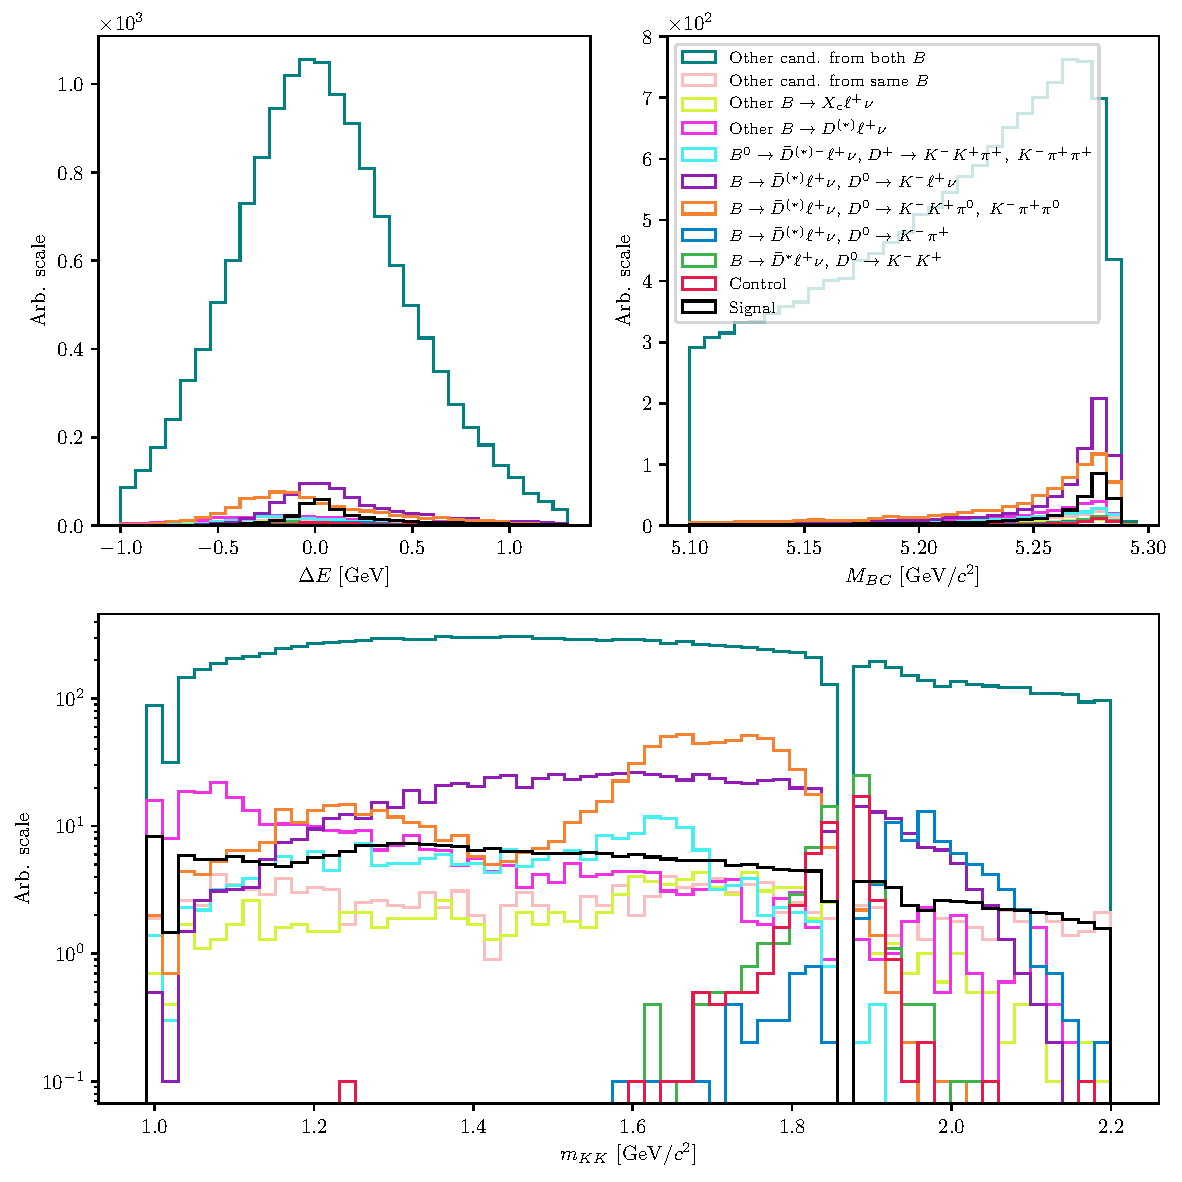
\includegraphics[width=\linewidth]{fig/sig_BKG_composition_all_before}
	\caption{Distributions of $\Delta E$ (left) and $M_{BC}$ (right) for various sources of the $B \bar B$ background after imposing the signal $KK$ invariant mass cut. The major source of the $B \bar B$ background comes from candidates with a $K\ell$ pair from one $B$ meson and the remaining $K$ from the other one.}
	\label{fig:sig_BKG_comp}
\end{figure}

\subsection{Templates in control fits}

In case of control sample fits the situation is similar. The difference is that in this case the yield of the control template was left as a floating parameter, while the yield of the signal template was fixed to the expected MC value for the same reasons as mentioned before. In this case, the following fit templates are chosen
\begin{itemize}
	\item signal template,
	\item control template,
	\item $B \to \bar D {}^* \ell^+ \nu$ template,
	\item other $B \bar B$ BKG template,
	\item $q \bar q$ template.
\end{itemize}
Since the background composition in the control region is different, we introduce a new category template for the background.  All sources of $B \bar B$ background for the control $KK$ invariant mass region are shown in Figure \ref{fig:cs_BKG_comp}.

\begin{figure}[H]
	\centering
	\captionsetup{width=0.8\linewidth}
	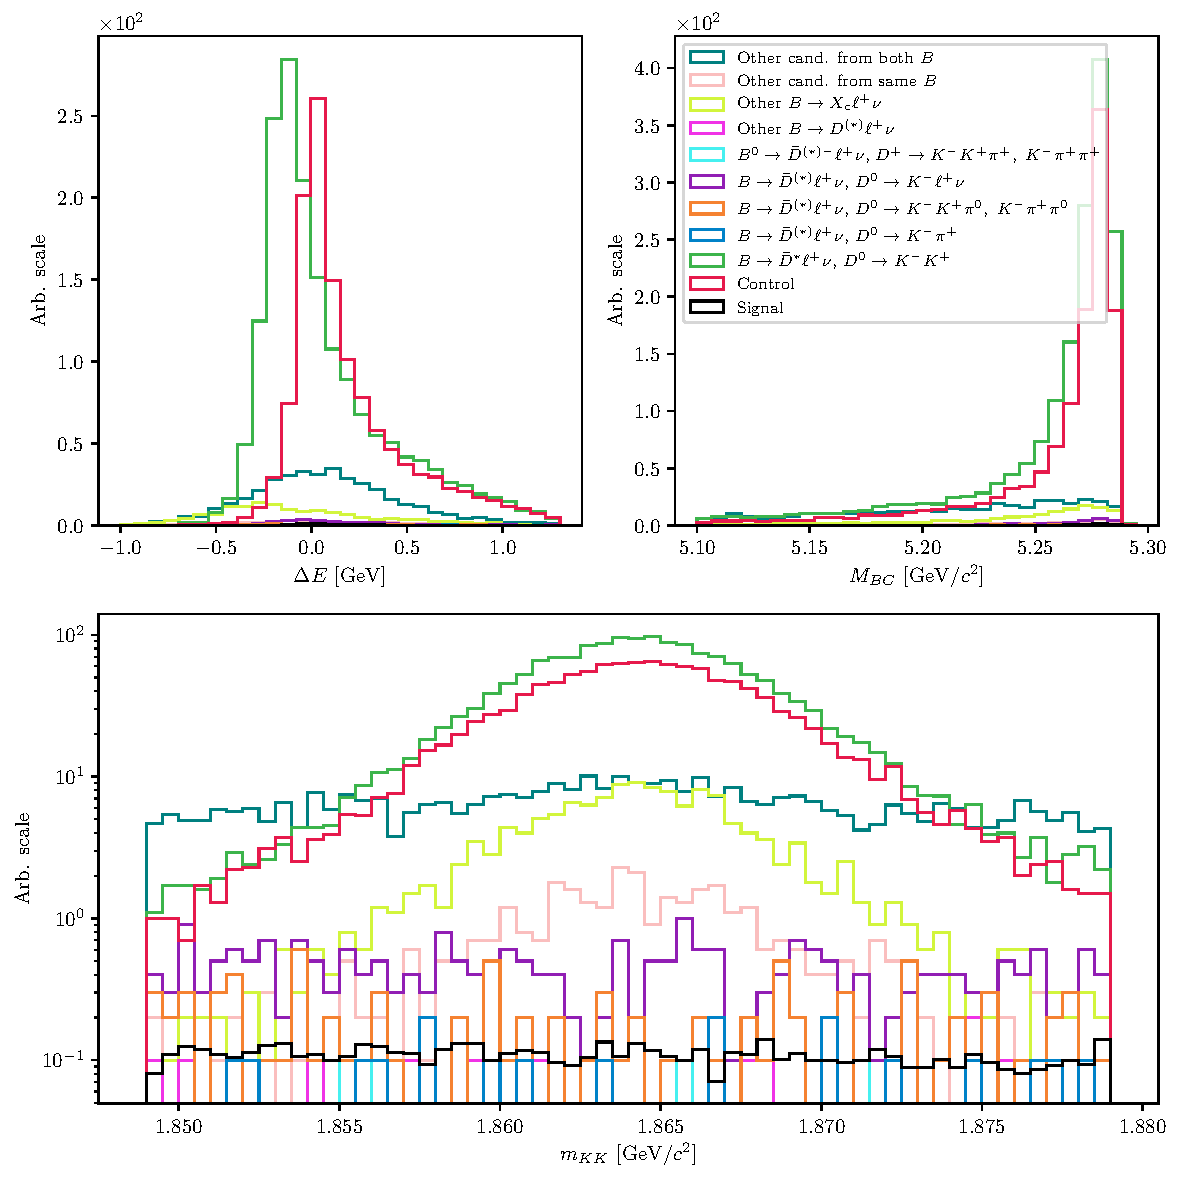
\includegraphics[width=\linewidth]{fig/cs_BKG_composition_before}
	\caption{Distributions of $\Delta E$ (left) and $M_{BC}$ (right) for various sources of the $B \bar B$ background after imposing the control $KK$ invariant mass cut. The major source of the $B \bar B$ background comes from candidates with a $K\ell$ pair from one $B$ meson and the remaining $K$ from the other one.}
	\label{fig:cs_BKG_comp}
\end{figure}

\section{Adaptive binning algorithm}\label{sec:adaptive-binning-algorithm}

The fit templates contain areas of low statistics, which are populated with bins with zero content. This is a direct consequence of having a finite MC sample and represent a liability in ML fits. Due to low statistic in the edge regions, the locations of these empty bins can vary for the templates and the fitted sample. A problem occurs if all templates have an empty bin where the fitted sample does not. In the scope of ML fits, this effectively means that there are entries in bins where the probability of having them is $0$. We will call such bins \textit{problematic}, because in these cases the fit does not converge.

The ideal solution for this problem would be to increase the MC statistics. Since this is not an option, we pursue other solutions, such as decreasing the number of bins. While this solves the problem, the drawback of it is a decrease in the template resolution in densely populated regions, where good resolution is most needed. The optimal solution here seems to be a choice of variable bins, with fine binning in the densely populated regions and larger bins in the regions with low statistics.

We have devised an algorithm, which compares the templates and the fitted sample, and defines a variable binning so that there are no more problematic bins in the end. Figure \ref{fig:adapt} shows an example of how the procedure works. The algorithm takes an argument for the initial number of uniform bins in each dimension, and does the following
\begin{enumerate}
\item define uniform binning in both dimensions with the provided argument,
\item create a 2D histogram from MC templates with expected yields,
\item define an \textit{optimal} region, where most of the 2D integral is contained and where all bins have a non-zero content (this region does not change throughout the process),
\item compare the histograms for the expected and the fitted sample, find the problematic bins,
\item loop until all problematic bins disappear
	\begin{enumerate}
	\item find problematic bin, which is nearest to the maximum bin,
	\item change the binning from $N$ to $N-1$ from that bin and in the direction away from the maximum bin.
	\end{enumerate}
\end{enumerate}

\begin{figure}[H]
	\centering
	\captionsetup{width=0.8\linewidth}
	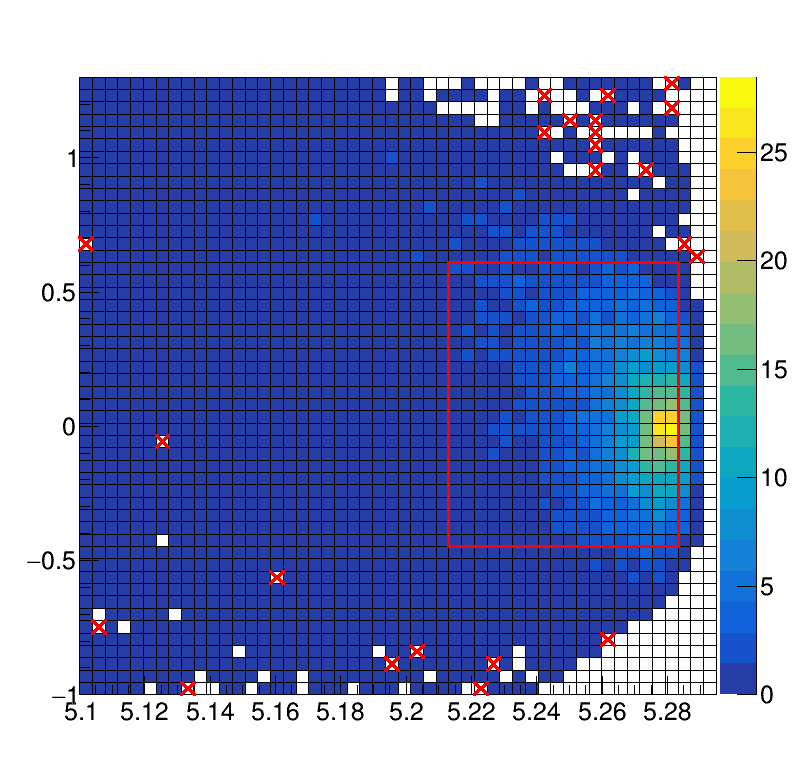
\includegraphics[width=0.49\linewidth]{fig/adaptive_1}
	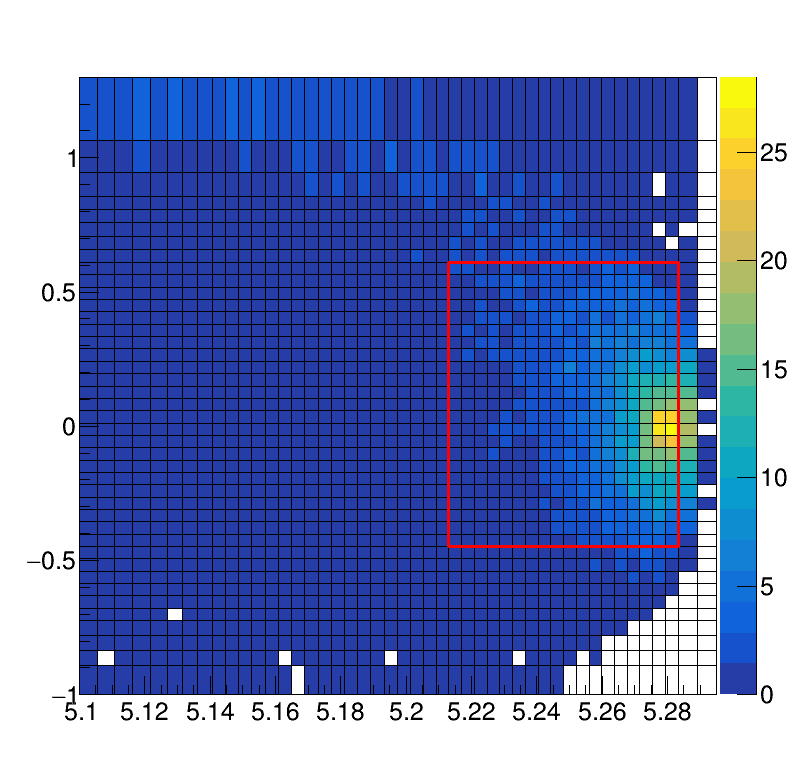
\includegraphics[width=0.49\linewidth]{fig/adaptive_15}
	\caption{Steps taken in the adaptive binning algorithm. Left image shows the initial 2D histogram with the defined optimal region and the problematic bins, the right image shows the final binning with the unchanged optimal region, while the problematic bins are gone due to the new binning choice.}
	\label{fig:adapt}
\end{figure}

An additional problem occurs in the plotting of the fitted templates and the sample with variable binning. It would seem that RooFit does not take the bin widths into account when plotting, while everything works as expected for the fit itself. This was bypassed by extracting the fitted yields and applying them to templates and samples with uniform binning, which were then used for drawing.

\section{Signal MC fit results}\label{sec:signal-mc-fit-results}

The fit setup was used on the final samples obtained with both versions of the final selection (standard BDT and uBDT). The choice of the initial uniform binning is not obvious, so we perform fits to all streams of MC for each initial binning choice and the fitted and expected yield difference, pulls and fit significance for both final samples, shown in Figure \ref{fig:sig_binning}. The difference between fitted an expected signal yield should be equal to 0 to ensure no bias is present in the fit, while the average pull distribution for each bin case should have a central value at 0, with a width of 1. Fits to final sample, obtained with the uBDT classifier generally seem to have a lower bias, pull distributions closer to the normal distribution and better significance than the fits in the case of the standard BDT final sample. This fixes our choice of the final selection. It is also possible to determine the optimal initial binning choice to be somewhere in the region of $20$ bins in each dimension, since a higher number of initial bins yields biased results, while a lower one yields results with poorer significance.

\begin{figure}[H]
	\centering
	\captionsetup{width=0.8\linewidth}
	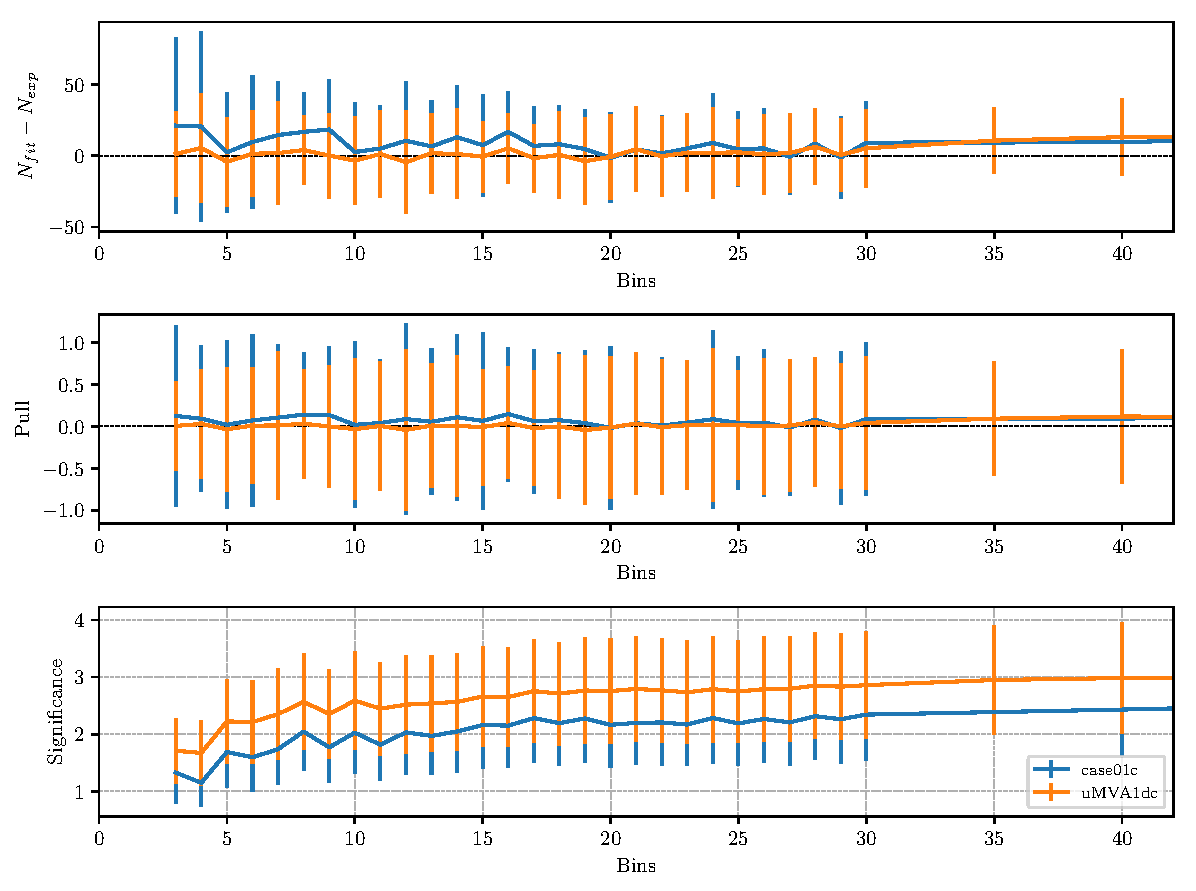
\includegraphics[width=\linewidth]{fig/sig_binning}
	\caption{Fitted yield and expected yield difference (top), pulls (center) and fit significance (bottom) as a function of binning in \vars~for the final sample, optimized with the standard BDT classifier (blue) and the uBDT classifier (orange).}
	\label{fig:sig_binning}
\end{figure}

Figure \ref{fig:sig_streamfit} shows the fit result and the fitted sample of an arbitrary stream for \vars, for the fit region and for the signal region. The fits seem stable and fit errors are under control. Fit results for all streams of MC are shown in Figure \ref{fig:sig_global}, along with the global fit of a zero degree polynomial over all streams. The results seem to describe the expected value in a precise manner, with the bias much smaller than the average statistical error. The normalized $\chi^2$ value with $10-1=9$ degrees of freedom of the global fit is $\chi^2_9 = 0.9$, while the average significance of the fits is around $3.17 \sigma$.

\begin{figure}[H]
	\centering
	\captionsetup{width=0.8\linewidth}
	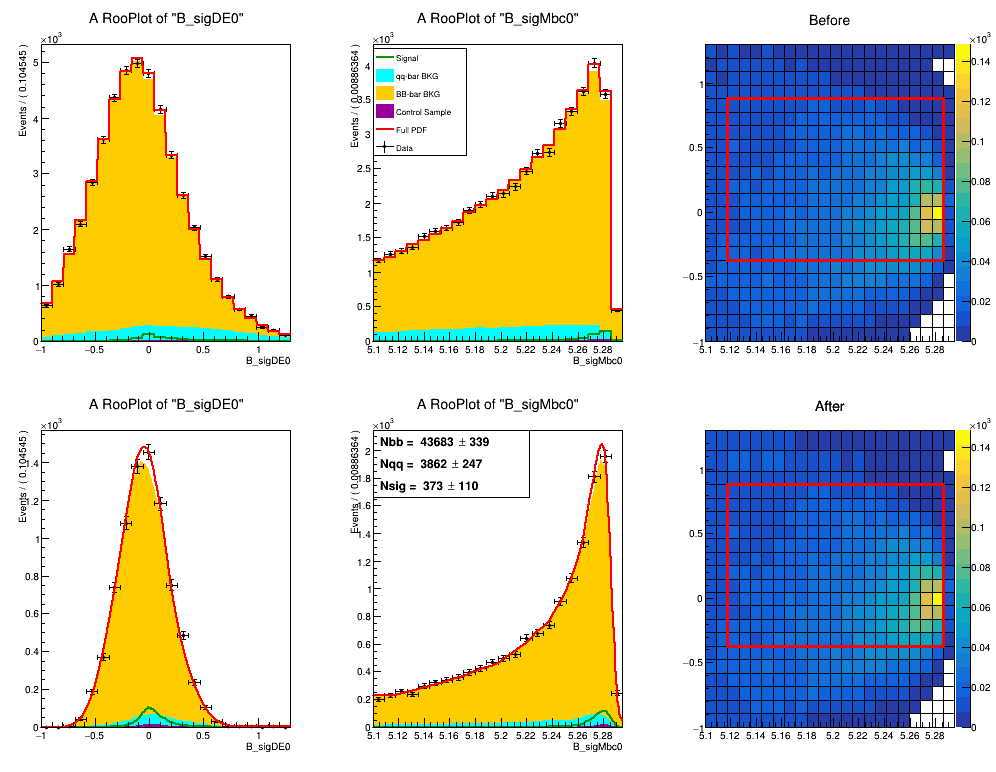
\includegraphics[width=\linewidth]{fig/plt_uMVA1dc_0.png}
	\caption{An example fit to one stream of MC. Left column shows the $M_{BC}$ and the center column shows the $\Delta E$ distribution of the full fitted sample in the full fit region (top) and the signal region (bottom). The right column shows the expected 2D histogram in \vars~with initial uniform binning (top) and the variable binning (bottom) after the binning algorithm.}
	\label{fig:sig_streamfit}
\end{figure}
%TODO fix fit plots


\begin{figure}[H]
	\centering
	\captionsetup{width=0.8\linewidth}
	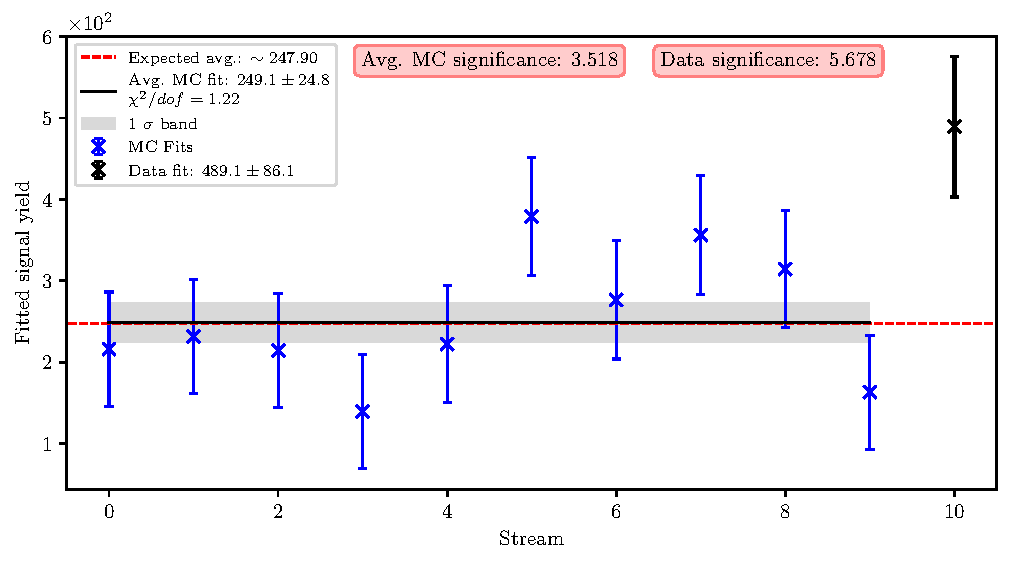
\includegraphics[width=\linewidth]{fig/sig_global}
	\caption{Fits to all 10 streams of MC and the global fit with a zero degree polynomial. The red like shows the mean value of the global fit and the green band shows the $1\sigma$ confidence interval. The expected value here differs slightly from the values in Section \ref{sec:selection-optimization}, since it is evaluated on a 10 stream sample size of the $20\times L_0$ \texttt{ulnu} sample.}
	\label{fig:sig_global}
\end{figure}

\subsection{Toy MC experiment}

Toy MC experiments allow us to study the yields, errors and the pulls of the signal fit by generating our own pseudo datasets, according to the MC, and not producing it in the standard way, which consumes unaffordable amounts of CPU time. In order to test the fit behavior, a toy MC study was performed where all available MC was used for template creation. We constructed $3\E{3}$ pseudo datasets, where each dataset was generated expected amount of each template category, distributed according to the Poisson distribution. All fits were performed with the optimal initial uniform binning of $20\times20$ bins in \vars.

Figure \ref{fig:toyMC} shows distributions of the fit yields, errors and the pull distribution of all pseudo fits. The fits seem to be under control since there is not any significant bias, and the pulls follow a normal distribution with a mean of $(1.1\pm1.8)\E{-2}$ and standard deviation of $(1.013\pm0.013)$. The mean ($\bar X$) and the standard deviation $(S)$ were calculated in the usual way, while the errors of these statistics were obtained by calculating the standard error of the mean ($\sigma_{\bar X}$) and standard deviation ($\sigma_S$), taken from \cite{ahn2003standard}, as
\begin{equation}
\sigma_{\bar X} = \frac{S}{\sqrt{N}},\quad \sigma_{S} = \frac{S}{\sqrt{2(N-1)}},
\end{equation}
where $N$ is the number of performed measurements.

\begin{figure}[H]
	\centering
	\captionsetup{width=0.8\linewidth}
	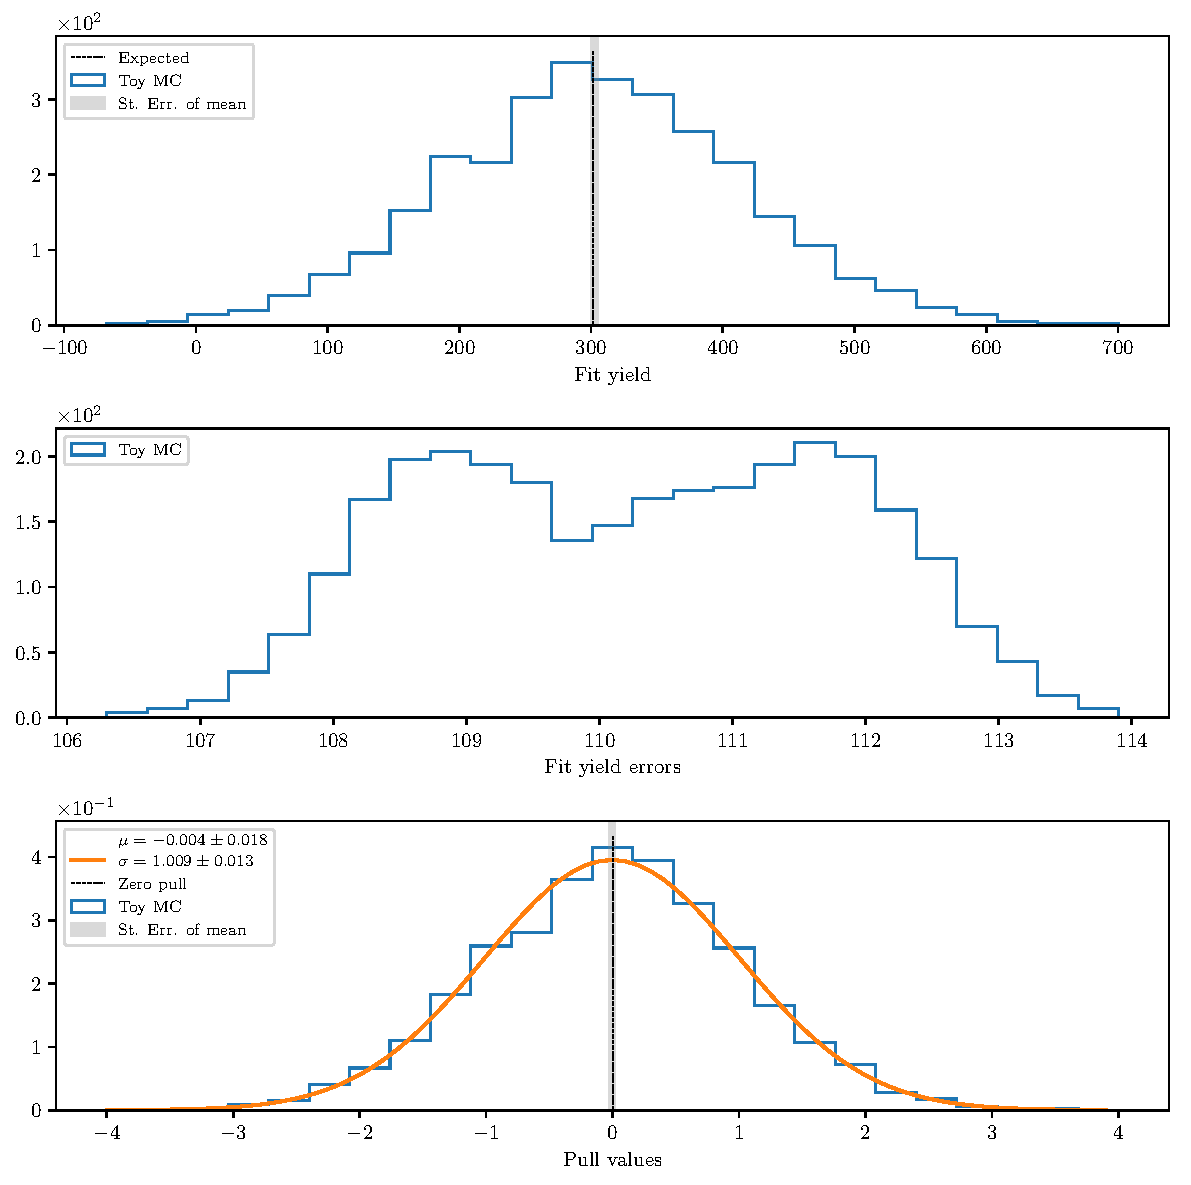
\includegraphics[width=\linewidth]{fig/toyMC}
	\caption{Toy MC fits of pseudo data showing the fit yield (top), fit errors (center) and the pull distribution of the fits (bottom).}
	\label{fig:toyMC}
\end{figure}

\subsection{Toy MC linearity test}
Linearity test is used for determining sensitivity of the fit to the amount of signal in the fitted sample. Since this is a first measurement of this decay channel, MC modeling is not reliable and could be very different from reality, so we need to perform this test in order to determine our sensitivity to smaller, as well as larger amounts of expected signal.

The pseudo datasets are generated in the same way as in the previous subsection, with the exception of signal, which is generated with various amounts. $50$ steps from $[0.1,~10]$ in the logarithmic scale are taken for fractions of signal amount and for each fraction we generate 500 pseudo datasets according to Poisson statistics.

Figure \ref{fig:lin_test} shows the mean fit yield and expected yield difference, mean pull and the mean significance at each signal fraction value. The expected MC result is shown at fraction value $1$. The plots show no significant bias with with respect to the signal fraction, while the pulls seems to be described by the normal distributions throughout the fraction range. At expected value we are at about $3.2\sigma$ significance, as already pointed out at the beginning of this section.

\begin{figure}[H]
	\centering
	\captionsetup{width=0.8\linewidth}
	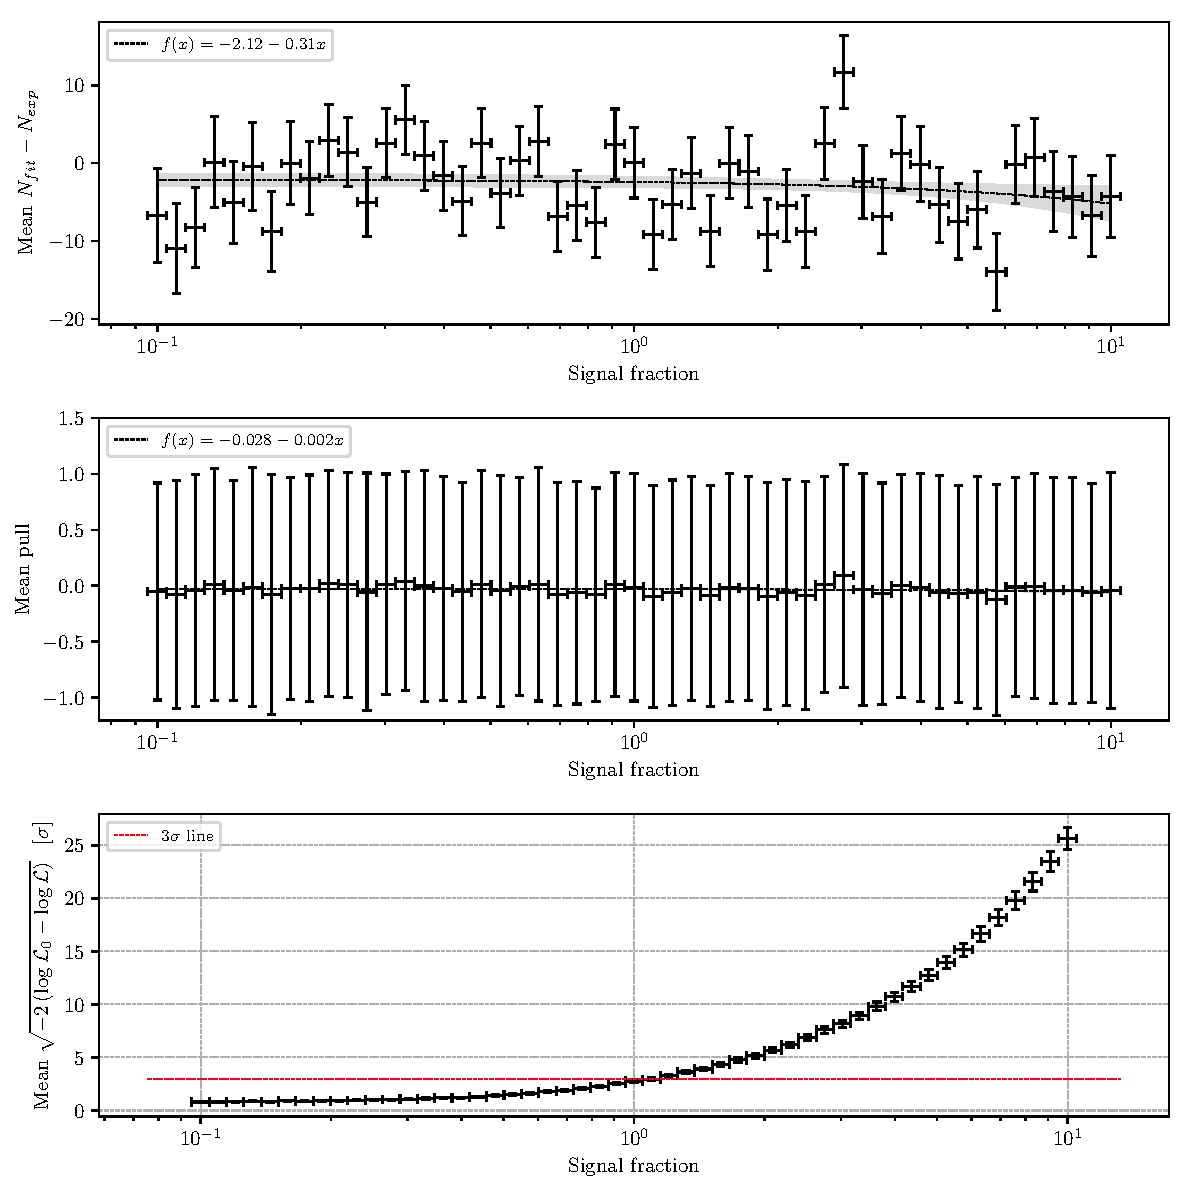
\includegraphics[width=\linewidth]{fig/lin_test}
	\caption{Mean fit yield and expected yield difference (top), mean pull (center) and mean significance (bottom) as a function of signal fraction.}
	\label{fig:lin_test}
\end{figure}

\section{Control fit results}

A similar fit procedure as in Section \ref{sec:signal-mc-fit-results} is applied in the case of the control decay on MC. In case of fits to real data, several corrections and constraints are applied before performing the fit

\begin{itemize}
%\item constraining the ratio between control and $B \to D^* \ell^+ \nu$,
\item a smearing factor to all MC templates,
\item an offset to all MC templates
\end{itemize}

\subsection{Smearing and offset parameters}

With simulated data we are able to perform detailed studies prior to looking at measured data. However, simulated data often does not describe data perfectly. Out of variables \vars, $\Delta E$ is especially prone to a lack of precision in energy measurements. This can introduce either overestimation of resolution on MC as well as a possible shift in the measured energy in either direction. Due to this fact, we perform a scan over additional 2 parameters of offset and smearing, applied on the $\Delta E$ variable. In case of the $M_{BC}$ variable the mentioned effects are not as prominent, so the smearing and offset for the latter variable are omitted. 

\subsubsection{Ratio constraint}

Introducing a smearing and offset factor can lead to unphysical global minima in the negative log-likelihood, where we mold a single MC template to almost perfectly describe data, while other contributions are rejected by the fit. In order to bypass this problem, we fix the ratio between the  $B \to \bar D {}^* \ell \nu$ sample and the control sample to the expected MC value in case of the MC fit, and to a corrected expected MC value for the data fit, where the corrections to the appropriate measured branching ratios are applied. In the latter case the constraint is applied in the form of a Gaussian function with the mean at the calculated value and with the width according to the appropriately propagated error.

The expected MC ratio and the corrected ratio are calculated as
\begin{align}
\eta_{MC} &= \frac{N^{MC}_{B \to \bar D {}^* \ell^+ \nu}}{N^{MC}_{\mathrm{control}}},\\
\eta_{DATA} &= \frac{N^{MC}_{B^+ \to \bar D {}^{*0} \ell^+ \nu}\times \rho_{B^+ \to \bar D {}^{*0} \ell^+ \nu} + N^{MC}_{B^0 \to D^{*-} \ell^+ \nu}\times \rho_{B^0 \to D^{*-} \ell^+ \nu}}{N^{MC}_{\mathrm{control}}\times \rho_{B^+ \to \bar D {}^{0} \ell^+ \nu}},
\label{eq:ratioData}
\end{align}
where each $\rho_X$ is defined as 
\begin{equation*}
\rho_X = \frac{\mathcal{B}_{PDG}(X)}{\mathcal{B}_{GEN}(X)},
\end{equation*}
and where the appropriate branching ratio values $\mathcal{B}_{PDG}$ and $\mathcal{B}_{GEN}$ are values taken from the PDG \cite{tanabashi2018review} and from tables used in MC generation, respectively. Table \ref{tab:br} shows the corresponding values of all mentioned branching ratios.

\begin{table}[H]
	\centering
\begin{tabular}{|l|c|c|}
	\hline
	Decay mode & $\mathcal{B}_{PDG}$ & $\mathcal{B}_{GEN}$ \\
	\hline
	$1)~B^+ \to \bar D {}^{*0} \ell^+ \nu$ & $(5.25\pm0.12)\E{-2}$ & $5.79\E{-2}$ \\
	$2)~B^0 \to D^{*-} \ell^+ \nu$ & $(4.88\pm0.11)\E{-2}$ & $5.33\E{-2}$ \\
	$3)~B^+ \to \bar D {}^0 \ell^+ \nu$ & $(2.29\pm0.10)\E{-2}$ & $2.31\E{-2}$ \\
	$4)~D^0 \to K^+ K^-$ & $(3.97\pm0.07)\E{-3}$ & $3.90\E{-3}$ \\
	\hline
	Control $3) \times 4)$ & $(9.10\pm0.42)\times 10^{-5}$ & $9.01\times 10^{-5}$ \\
	\hline
\end{tabular}
	\caption{Generated and PDG branching ratios of several decay modes.}
	\label{tab:br}
\end{table}

Finally, after calculating the ratio and propagating the statistical errors and errors of the measurements, we obtain
\begin{align*}
\eta_{MC} &= 1.41,\\
\eta_{DATA} &= 1.29\pm 0.06,
\end{align*}
where errors of all terms in Eq. (\ref{eq:ratioData}) were assumed to be uncorrelated, except for errors of $\rho_{B^+ \to \bar D {}^{*0} \ell^+ \nu}$ and $\rho_{B^0 \to D^{*0} \ell^+ \nu}$, where we assumed $100\%$ error correlation, due to both values being obtained from the same measurement, assuming isospin symmetry.

\subsubsection{Determination of optimal parameters}

After fixing the ratio defined in previous subsubsection, we scan the following phase space
\begin{itemize}
\item smearing factor in range $[0.0,0.08]\e{GeV}$ in steps of $8\E{-3}$,
\item offset in range $[0.0,0.003]\e{GeV}$ in steps of $1.5\E{-3}$,
\end{itemize}
where for each parameter pair the likelihood ratio test is performed to estimate the goodness of the fit. Figure \ref{fig:smearing_offset} shows the contour plot of the likelihood ratio $\lambda$, as defined in Eq. (\ref{eq:lr}), for 2 d.o.f., for MC (left) and data (right). The scan over MC serves the purpose of a consistency check, where we expect the best fit to occur in the phase space where neither smearing nor offset are applied. In case of data, we see that we obtain a better fit by introducing some level of smearing and offset. The likelihood ratio test allows us to estimate the parameter values in the $1\sigma$ confidence interval, where we obtain the optimal parameter set
\begin{itemize}
\item Smearing: $24\e{MeV} \pm X$,
\item Offset: $6\e{MeV} \pm X$.
\end{itemize}
We apply this transformation to our MC samples in all cases when we fit real data.

\begin{figure}[H]
	\centering
	\captionsetup{width=0.8\linewidth}
	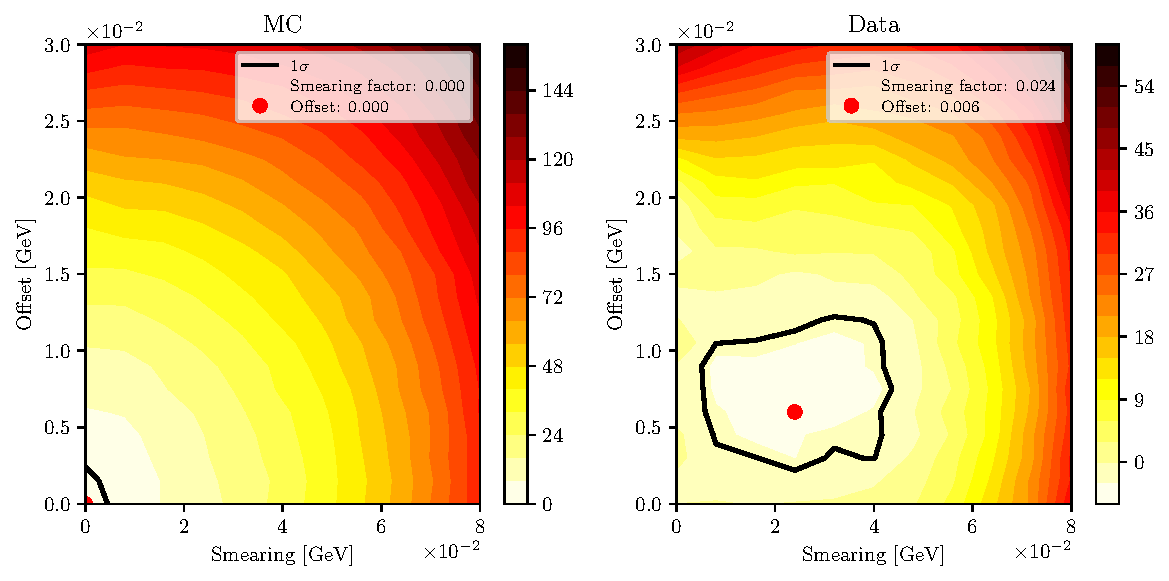
\includegraphics[width=\linewidth]{fig/smearing_offset}
	\caption{Likelihood ratio test of an additional smearing and offset parameter to MC (left) and data (right).}
	\label{fig:smearing_offset}
\end{figure}

\subsection{Consistency of MVA cuts}

Control sample fits allow us to check the behavior of optimized MVA cuts on MC as well as data and see if any of the MVA steps introduce a possible disagreement between the two. We compare control yields, their ratios and ratios of cut efficiencies (double ratios). The following cut scenarios are studied
\begin{itemize}
\item[(a)] final selection before any MVA step,
\item[(b)] (a) + $BDT_{q\bar q}$ cut,
\item[(c)] (a) + $uBDT_{B\bar B}$ cut,
\item[(d)] (a) + $BDT_{q\bar q} + uBDT_{B\bar B}$ cut (final selection).
\end{itemize}

The same binning was chosen as in the case of signal MC fits. The results for control fit yields, their ratios and double ratios are shown in Figure \ref{fig:cs_fits}. The plot shows that yield ratios and cut efficiency ratios are consistent with $1$. This means that, for the control sample, data and MC are in agreement before as well as after applying the final selection cuts. This is an important check for the signal decay mode, since, this check serves as an argument that the final selection is not over-optimized to signal MC.

\begin{figure}[H]
	\centering
	\captionsetup{width=0.8\linewidth}
	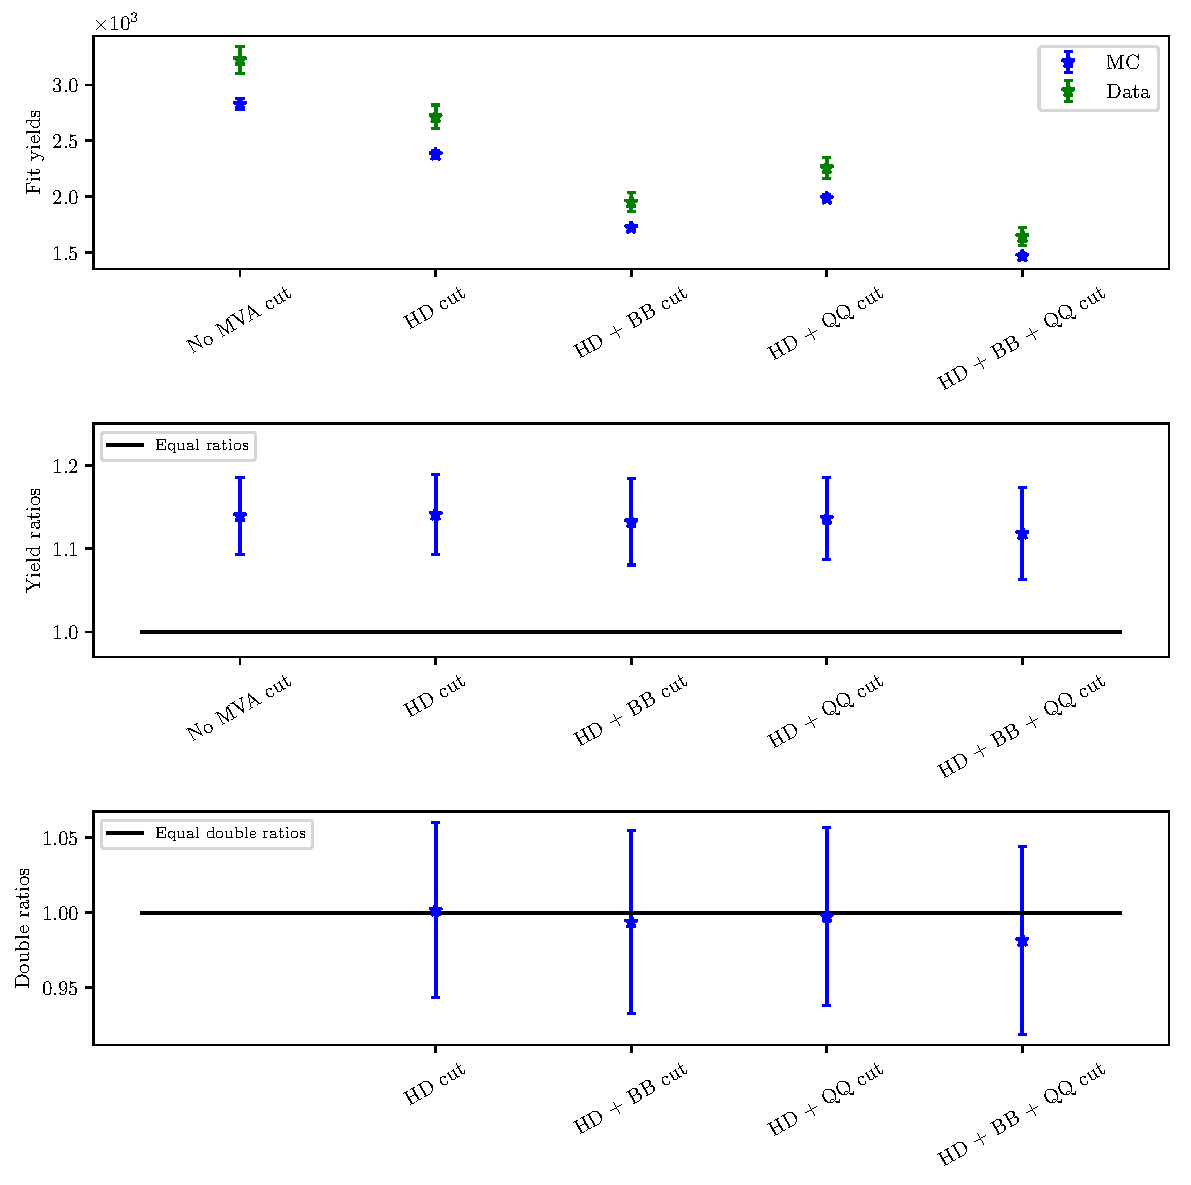
\includegraphics[width=\linewidth]{fig/cs_fits.pdf}
	\caption{Fit yields, their ratios and ratios of cut efficiencies (double ratios) for the control sample fits to data and MC.}
	\label{fig:cs_fits}
\end{figure}

\subsection{Control decay branching ratio measurement}

After acquiring the fit results on MC and data we are able to determine the branching ratio of the control decay on MC and data, which are defined as
\begin{align}
\mathcal{B}^{MC}_{\mathrm{control}} &= \frac{N^{\mathrm{MC}}_\mathrm{control} \times \epsilon_{MC}}{2N_{B\bar B}^{MC}},\\
\mathcal{B}_{\mathrm{control}} &= \frac{N_\mathrm{control} \times \epsilon_{MC} \times \rho_{PID}}{2N_{B\bar B}},
\label{eq:br_data}
\end{align}
where $N^{\mathrm{MC}}_\mathrm{control}$ and $N_\mathrm{control}$ are yields of the control fit on MC and data, $\epsilon_{MC}$ is the MC efficiency of the control sample, $\rho_{PID}$ the PID correction factor, and $N_{B\bar B}^{MC}$ and $N_{B\bar B}$ are the numbers of $B \bar B$ meson pairs on MC and in data, respectively. The factor of 2 in the denominator comes from the fact that there are 2 $B$ mesons in each $B$ meson pair $(\times 1/2)$, where only about $50\%$ of the $B$ meson pairs are charged $B^+B^-$ meson pairs $(\times 2)$, and from the fact that we are interested in the branching ratio to the lepton final state of either $e$ or $\mu$, and not their sum $(\times 1/2)$.

The control sample efficiency was determined on a separate signal MC sample of the control decay, where we generated $5\E{6}$ $B^+ \bar B^-$ pairs, with one $B$ always decaying via $B^+ \to \bar D {}^0 \ell^+ \nu,~D^0 \to K^+K^-$. After applying the final selection, the full and split efficiencies with regard to the lepton final state were determined to be 
\begin{align*}
\epsilon_{MC} &= (8.89\pm 0.04)\E{-3},\\
\epsilon_{MC}^e &= (4.40\pm 0.03)\E{-3},\\
\epsilon_{MC}^\mu &= (4.49\pm 0.03)\E{-3},
\end{align*}
where the efficiency error was estimated based on a formula from [X]
\begin{equation*}
\epsilon_{MC} = \frac{1}{N}\sqrt{n(1-\frac{n}{N})},
\end{equation*}
where $n$ is a subset of the full set $N$.

The PID correction factor is obtained by taking into account the known PID efficiency differences between data and MC. It is described in detail in X and is determined to be
\begin{equation*}
\rho_{PID} = 0.99\pm 0.02
\end{equation*}
for the $e$ and $\mu$ mode, as well both of them together.

The number of $B\bar B$ meson pairs can be counted on MC and has been measured for data [X]. The values are
\begin{align*}
&N_{B\bar B}^{MC} = 765.98\E{6},\\
&N_{B\bar B} = (771.58 \pm 10.56)\E{6}.
\end{align*}

The yields of control sample candidates and their errors were taken from the fits to MC and data. In case of MC, the fit results were averaged over 10 streams, which results in a smaller error. The fit results after the final selection are shown in Table \ref{tab:fit_yield}.

\begin{table}[H]
	\centering
	\begin{tabular}{|l|c|c|}
\hline
 & $N^{MC}$ & $N^{\mathrm{data}}$ \\
\hline
$\ell = e$ or $\mu$ & $1214.76 \pm 22.76$ & $1245.38 \pm 69.73$\\
	\hline
$\ell = e$ & $607.59 \pm 15.18$ & $602.74 \pm 47.32$ \\
\hline
$\ell = \mu$ & $607.34 \pm 12.39$ & $631.70 \pm 50.06$\\
	\hline
\end{tabular}
\caption{Control sample fit results for MC and data for various lepton final state modes.}
\label{tab:fit_yield}
\end{table}

Finally, we can determine the branching ratios based on the calculations in Eq. (\ref{eq:br_data}). The obtained values are shown in Table \ref{tab:br_result} and graphically shown in Figure \ref{fig:br_plot}, along with the MC generated value and the current PDG world average. Both MC and measured determination of the control decay branching ratio are in agreement with the expected and the world average values.

\begin{table}[H]
	\centering
	\begin{tabular}{|l|c|c|}
		\hline
		$\mathcal{B}_{PDG}$ & \multicolumn{2}{c|}{$(9.10\pm0.42)\E{-5}$} \\
		\hline
     	$\mathcal{B}_{GEN}$ & \multicolumn{2}{c|}{$9.01\E{-5}$} \\
     	\hline
		& $\mathcal{B}^{MC}$ & $\mathcal{B}^{\mathrm{data}}$ \\
		\hline
		$\ell = e$ or $\mu$ & $(8.92\pm0.17)\E{-5}$ & $(9.17\pm0.56)\E{-5}$\\
		\hline
		$\ell = e$ & $(9.02\pm0.23)\E{-5}$ & $(9.01\pm0.75)\E{-5}$ \\
		\hline
		$\ell = \mu$ & $(8.82\pm0.19)\E{-5}$ & $(9.17\pm0.77)\E{-5}$\\
		\hline
	\end{tabular}
	\caption{Control sample fit results for MC and data for various lepton final state modes.}
	\label{tab:br_result}
\end{table}

\begin{figure}[H]
	\centering
	\captionsetup{width=0.8\linewidth}
	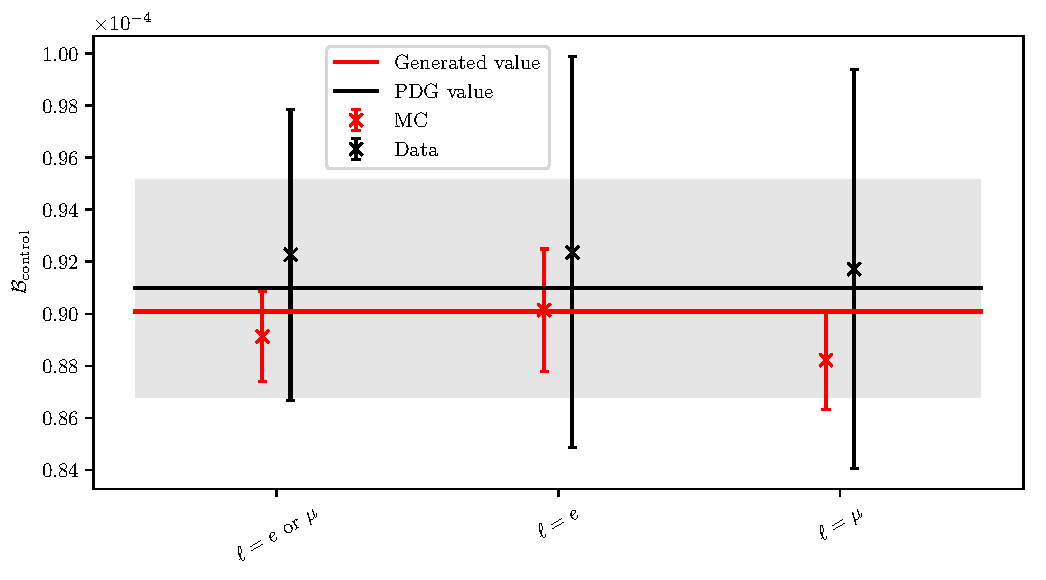
\includegraphics[width=\linewidth]{fig/br_plot}
	\caption{Various branching ratio determinations for the control decay of our analysis.}
	\label{fig:br_plot}
\end{figure}

\section{Signal fit to data}